\section{Experimental Results and Analysis}

\subsection{Hyperparameter Selection}

For each model, we selected the hyperparameter set 
that achieved the highest average accuracy 
over the 6-fold cross-validation. 

Once the best hyperparameters for each model were 
identified, we employed the Wilcoxon test to determine 
whether the differences between the average accuracies 
of the models were statistically significant. 
This step ensured that the observed differences 
were not due to random variation. 

Finally, we compared the best results obtained from 
the three models (Decision Tree, Random Forest, and Neural Network) 
to assess which model exhibited the 
highest overall performance.

\subsubsection{Decision Tree Results}

The Decision Tree model was evaluated with various 
hyperparameters. Among the configurations tested, 
the best performance was achieved with a maximum 
depth of 1000, using the "gini" criterion and a minimum 
impurity decrease of 0.0. 
This setting resulted in the highest average accuracy 
of approximately 0.4578. The models using the "entropy" 
criterion and "log\_loss" criterion with a maximum 
depth of 1000 also performed well, with accuracies 
around 0.4199 and 0.4136, respectively. 
On the other hand, configurations with a maximum depth 
of \textit{null} and "entropy" or "log\_loss" criteria 
yielded lower accuracies, indicating that deeper trees 
tend to generalize better in this scenario.

\begin{figure}[H]
    \centering
    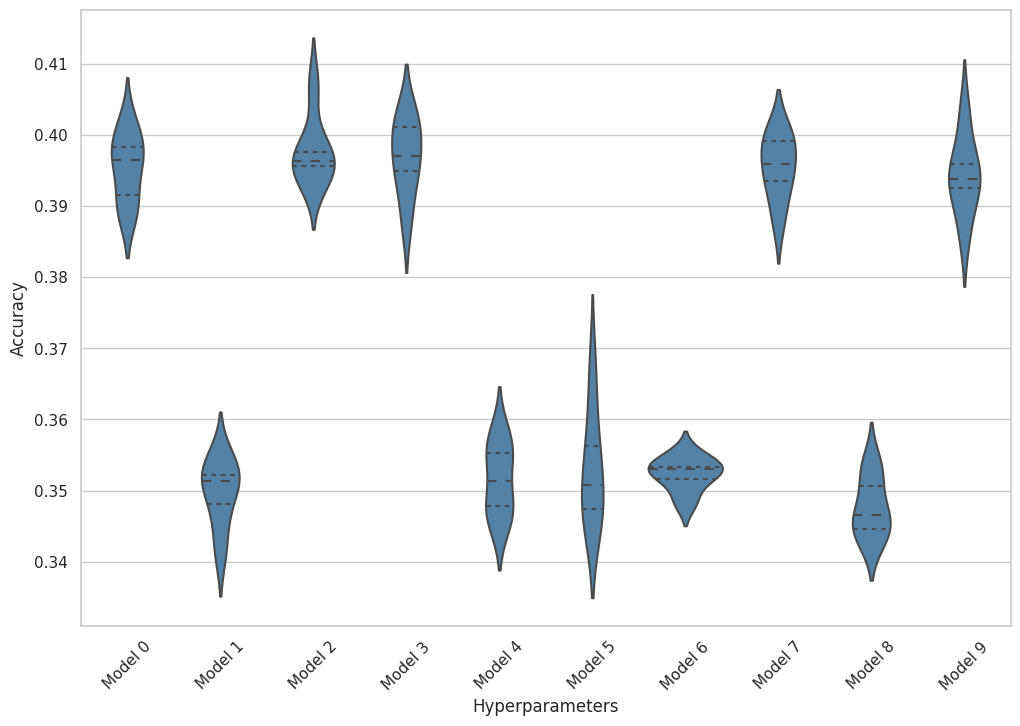
\includegraphics[width=0.99\columnwidth]{images/violin_plot_decision_tree.png}
    \caption{Accuracy distribution for Decision Trees}
    \label{fig:dt_violin_plot}
\end{figure}

\subsubsection{Random Forest Results}

The Random Forest model demonstrated its best performance 
with a configuration of 100 estimators, "gini" criterion, 
and a maximum depth of \textit{null}. 
This setup achieved the highest average accuracy of 
approximately 0.6267. 
Other effective configurations included 100 estimators 
with the "gini" criterion and a maximum depth of 1000, 
reaching an accuracy of around 0.6241. 
The "log\_loss" criterion with 150 estimators also 
performed well but was slightly less accurate compared 
to the "gini" based configurations. 
Conversely, models with fewer estimators or different 
criteria, such as "entropy," generally resulted 
in lower accuracies. This indicates that increasing 
the number of estimators and optimizing depth are 
crucial for improving performance in 
Random Forest models.

\begin{figure}[H]
    \centering
    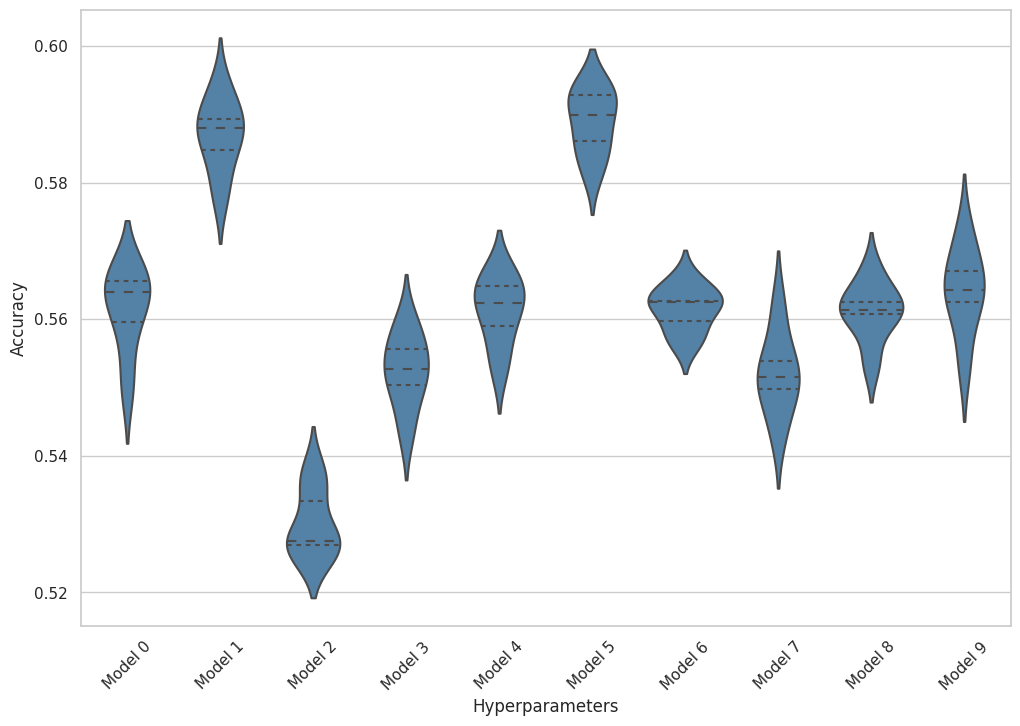
\includegraphics[width=0.99\columnwidth]{images/violin_plot_random_forest.png}
    \caption{Accuracy distribution for Random Forests}
    \label{fig:rf_violin_plot}
\end{figure}

\subsubsection{Neural Network Results}

For the Neural Network models, the configurations 
with a hidden size of 64 and learning rates of 0.005 
or 0.01 yielded the highest average accuracies. 
Specifically, the setting with 64 hidden units, 
10 epochs, and a learning rate of 0.005 achieved 
an accuracy of around 0.6097, while another setting 
with the same hidden size and learning rate of 0.01 
resulted in an accuracy of approximately 0.6136. 
The best performance was observed with a configuration 
of 64 hidden units, 5 epochs, and a learning rate of 0.001, 
achieving an accuracy of 0.6311. 
In contrast, models with smaller hidden sizes 
and shorter epochs generally showed lower performance, 
suggesting that deeper networks with more training epochs 
are more effective in capturing complex patterns.

\begin{figure}[H]
    \centering
    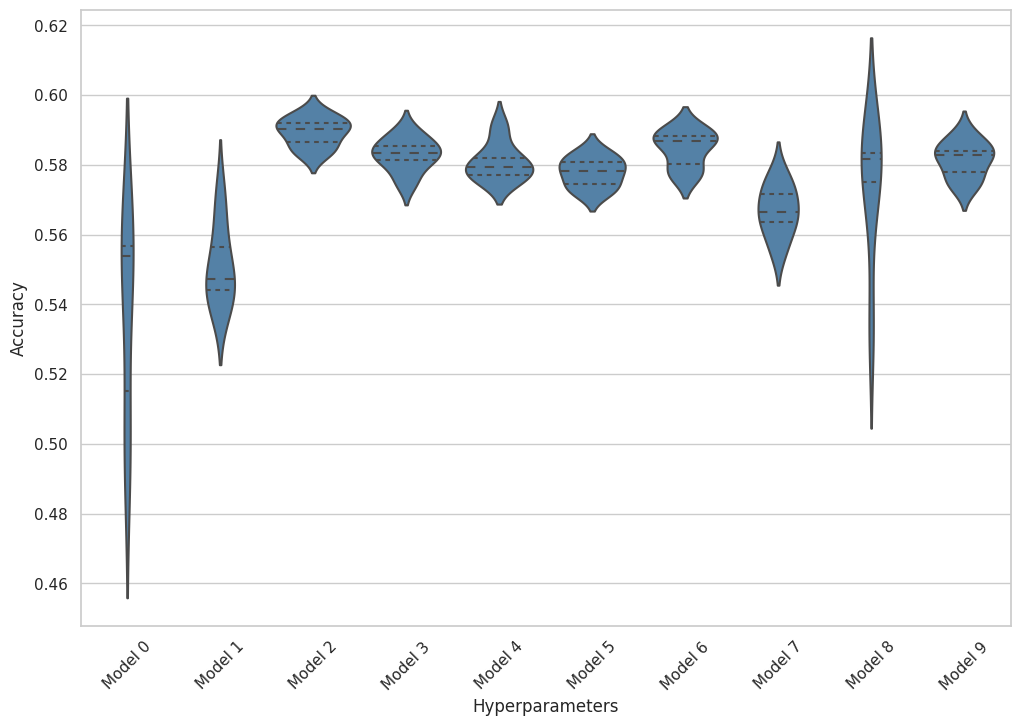
\includegraphics[width=0.99\columnwidth]{images/violin_plot_neural_network.png}
    \caption{Accuracy distribution for Neural Network}
    \label{fig:nn_violin_plot}
\end{figure}

\begin{table*}
    \centering
    \begin{tabular}{@{}cccc@{}}
        \toprule
        \textbf{Index} & \textbf{Criterion} & \textbf{Min Impurity Decrease} & \textbf{Max Depth} \\ \midrule
        0 & gini & 1e-10 & 200 \\
        1 & log\_loss & 1e-08 & 200 \\
        2 & gini & 1e-08 & 200 \\
        3 & gini & 1e-08 & 150 \\
        4 & log\_loss & 1e-10 & None \\
        5 & log\_loss & 0.0 & 150 \\
        6 & log\_loss & 0.0 & None \\
        7 & gini & 1e-10 & 150 \\
        8 & log\_loss & 1e-12 & 200 \\
        9 & gini & 0.0 & 200 \\ \bottomrule
    \end{tabular}
    \caption{Hyperparameters for Decision Tree}
    \label{tab:dt_search_spaces}
\end{table*}


\begin{table*}
    \centering
    \begin{tabular}{@{}ccccc@{}}
        \toprule
        \textbf{Index} & \textbf{Estimators} & \textbf{Criterion} & \textbf{Min Impurity Decrease} & \textbf{Max Depth} \\ \midrule
        0 & 50 & gini & 0.0 & None \\
        1 & 150 & gini & 0.0 & 200 \\
        2 & 50 & log\_loss & 1e-12 & 150 \\
        3 & 100 & log\_loss & 0.0 & 200 \\
        4 & 150 & log\_loss & 0.0 & 150 \\
        5 & 150 & gini & 0.0 & 150 \\
        6 & 150 & log\_loss & 1e-12 & 150 \\
        7 & 100 & log\_loss & 1e-12 & 150 \\
        8 & 50 & gini & 0.0 & 200 \\
        9 & 50 & gini & 1e-10 & 150 \\ \bottomrule
    \end{tabular}
    \caption{Hyperparameters for Random Forest}
    \label{tab:rf_search_spaces}
\end{table*}

\begin{table*}
    \centering
    \begin{tabular}{@{}ccccc@{}}
        \toprule
        \textbf{Index} & \textbf{Hidden Size} & \textbf{Epochs} & \textbf{Learning Rate} \\ \midrule
        0 & 16 & 8 & 0.0005 \\
        1 & 16 & 10 & 0.001 \\
        2 & 64 & 8 & 0.0005 \\
        3 & 32 & 6 & 0.0005 \\
        4 & 64 & 6 & 0.001 \\
        5 & 64 & 8 & 0.001 \\
        6 & 64 & 10 & 0.0005 \\
        7 & 64 & 6 & 0.005 \\
        8 & 32 & 6 & 0.001 \\
        9 & 32 & 10 & 0.0005 \\ \bottomrule
    \end{tabular}
    \caption{Hyperparameters for Neural Network}
    \label{tab:nn_search_spaces}
\end{table*}


\subsection{Best Model Comparison}

Among the evaluated models, the Neural Network (NN) 
configuration with 64 hidden units, 5 epochs, and a 
learning rate of 0.001 achieved the highest average 
accuracy of approximately 0.6244. 
This model demonstrates strong performance, 
particularly in its ability to capture complex patterns 
within the data. The Random Forest (RF) model, with 100 
estimators, "gini" criterion, and a maximum depth 
of 1000, also performed impressively, attaining an 
average accuracy of around 0.6219. 
Although slightly lower than the NN, it remains a 
robust model for classification tasks. 
The Decision Tree (DT) model, using the "gini" criterion, 
a minimum impurity decrease of 1e-08, and a maximum 
depth of 1000, had an average accuracy of about 0.4579. 
While this accuracy is significantly lower than that 
of the RF and NN models, it is important to note that 
Decision Trees are generally less effective on their 
own compared to ensemble methods and neural networks. 
Overall, the Neural Network achieved the highest 
performance, followed closely by the Random Forest, 
while the Decision Tree showed comparatively lower 
results.

